%\documentclass[3p, twocolumn, sort&compress]{elsarticle}
\documentclass[aps,tightenlines,superscriptaddress,twocolumn]{revtex4-1}
\usepackage{graphicx}
\usepackage{bm}
\usepackage{times}
\usepackage{lineno}
\usepackage[pscoord]{eso-pic}

\begin{document}

\title{Probing Strangeness Canonical Ensemble with $K^{-}$, $\phi(1020)$ and $\Xi^{-}$ Production in Au+Au Collisions at ${\sqrt{s_{\rm NN}} = \rm{3\,GeV}}$: Supplemental Material}% Force line breaks with \\

\affiliation{Abilene Christian University, Abilene, Texas   79699}
\affiliation{AGH University of Science and Technology, FPACS, Cracow 30-059, Poland}
\affiliation{Alikhanov Institute for Theoretical and Experimental Physics NRC "Kurchatov Institute", Moscow 117218}
\affiliation{Argonne National Laboratory, Argonne, Illinois 60439}
\affiliation{American University of Cairo, New Cairo 11835, New Cairo, Egypt}
\affiliation{Brookhaven National Laboratory, Upton, New York 11973}
\affiliation{University of California, Berkeley, California 94720}
\affiliation{University of California, Davis, California 95616}
\affiliation{University of California, Los Angeles, California 90095}
\affiliation{University of California, Riverside, California 92521}
\affiliation{Central China Normal University, Wuhan, Hubei 430079 }
\affiliation{University of Illinois at Chicago, Chicago, Illinois 60607}
\affiliation{Creighton University, Omaha, Nebraska 68178}
\affiliation{Czech Technical University in Prague, FNSPE, Prague 115 19, Czech Republic}
\affiliation{Technische Universit\"at Darmstadt, Darmstadt 64289, Germany}
\affiliation{ELTE E\"otv\"os Lor\'and University, Budapest, Hungary H-1117}
\affiliation{Frankfurt Institute for Advanced Studies FIAS, Frankfurt 60438, Germany}
\affiliation{Fudan University, Shanghai, 200433 }
\affiliation{University of Heidelberg, Heidelberg 69120, Germany }
\affiliation{University of Houston, Houston, Texas 77204}
\affiliation{Huzhou University, Huzhou, Zhejiang  313000}
\affiliation{Indian Institute of Science Education and Research (IISER), Berhampur 760010 , India}
\affiliation{Indian Institute of Science Education and Research (IISER) Tirupati, Tirupati 517507, India}
\affiliation{Indian Institute Technology, Patna, Bihar 801106, India}
\affiliation{Indiana University, Bloomington, Indiana 47408}
\affiliation{Institute of Modern Physics, Chinese Academy of Sciences, Lanzhou, Gansu 730000 }
\affiliation{University of Jammu, Jammu 180001, India}
\affiliation{Joint Institute for Nuclear Research, Dubna 141 980}
\affiliation{Kent State University, Kent, Ohio 44242}
\affiliation{University of Kentucky, Lexington, Kentucky 40506-0055}
\affiliation{Lawrence Berkeley National Laboratory, Berkeley, California 94720}
\affiliation{Lehigh University, Bethlehem, Pennsylvania 18015}
\affiliation{Max-Planck-Institut f\"ur Physik, Munich 80805, Germany}
\affiliation{Michigan State University, East Lansing, Michigan 48824}
\affiliation{National Research Nuclear University MEPhI, Moscow 115409}
\affiliation{National Institute of Science Education and Research, HBNI, Jatni 752050, India}
\affiliation{National Cheng Kung University, Tainan 70101 }
\affiliation{Nuclear Physics Institute of the CAS, Rez 250 68, Czech Republic}
\affiliation{Ohio State University, Columbus, Ohio 43210}
\affiliation{Institute of Nuclear Physics PAN, Cracow 31-342, Poland}
\affiliation{Panjab University, Chandigarh 160014, India}
\affiliation{Pennsylvania State University, University Park, Pennsylvania 16802}
\affiliation{NRC "Kurchatov Institute", Institute of High Energy Physics, Protvino 142281}
\affiliation{Purdue University, West Lafayette, Indiana 47907}
\affiliation{Rice University, Houston, Texas 77251}
\affiliation{Rutgers University, Piscataway, New Jersey 08854}
\affiliation{Universidade de S\~ao Paulo, S\~ao Paulo, Brazil 05314-970}
\affiliation{University of Science and Technology of China, Hefei, Anhui 230026}
\affiliation{Shandong University, Qingdao, Shandong 266237}
\affiliation{Shanghai Institute of Applied Physics, Chinese Academy of Sciences, Shanghai 201800}
\affiliation{Southern Connecticut State University, New Haven, Connecticut 06515}
\affiliation{State University of New York, Stony Brook, New York 11794}
\affiliation{Instituto de Alta Investigaci\'on, Universidad de Tarapac\'a, Arica 1000000, Chile}
\affiliation{Temple University, Philadelphia, Pennsylvania 19122}
\affiliation{Texas A\&M University, College Station, Texas 77843}
\affiliation{University of Texas, Austin, Texas 78712}
\affiliation{Tsinghua University, Beijing 100084}
\affiliation{University of Tsukuba, Tsukuba, Ibaraki 305-8571, Japan}
\affiliation{Valparaiso University, Valparaiso, Indiana 46383}
\affiliation{Variable Energy Cyclotron Centre, Kolkata 700064, India}
\affiliation{Warsaw University of Technology, Warsaw 00-661, Poland}
\affiliation{Wayne State University, Detroit, Michigan 48201}
\affiliation{Yale University, New Haven, Connecticut 06520}

\author{M.~S.~Abdallah}\affiliation{American University of Cairo, New Cairo 11835, New Cairo, Egypt}
\author{B.~E.~Aboona}\affiliation{Texas A\&M University, College Station, Texas 77843}
\author{J.~Adam}\affiliation{Brookhaven National Laboratory, Upton, New York 11973}
\author{L.~Adamczyk}\affiliation{AGH University of Science and Technology, FPACS, Cracow 30-059, Poland}
\author{J.~R.~Adams}\affiliation{Ohio State University, Columbus, Ohio 43210}
\author{J.~K.~Adkins}\affiliation{University of Kentucky, Lexington, Kentucky 40506-0055}
\author{G.~Agakishiev}\affiliation{Joint Institute for Nuclear Research, Dubna 141 980}
\author{I.~Aggarwal}\affiliation{Panjab University, Chandigarh 160014, India}
\author{M.~M.~Aggarwal}\affiliation{Panjab University, Chandigarh 160014, India}
\author{Z.~Ahammed}\affiliation{Variable Energy Cyclotron Centre, Kolkata 700064, India}
\author{I.~Alekseev}\affiliation{Alikhanov Institute for Theoretical and Experimental Physics NRC "Kurchatov Institute", Moscow 117218}\affiliation{National Research Nuclear University MEPhI, Moscow 115409}
\author{D.~M.~Anderson}\affiliation{Texas A\&M University, College Station, Texas 77843}
\author{A.~Aparin}\affiliation{Joint Institute for Nuclear Research, Dubna 141 980}
\author{E.~C.~Aschenauer}\affiliation{Brookhaven National Laboratory, Upton, New York 11973}
\author{M.~U.~Ashraf}\affiliation{Central China Normal University, Wuhan, Hubei 430079 }
\author{F.~G.~Atetalla}\affiliation{Kent State University, Kent, Ohio 44242}
\author{A.~Attri}\affiliation{Panjab University, Chandigarh 160014, India}
\author{G.~S.~Averichev}\affiliation{Joint Institute for Nuclear Research, Dubna 141 980}
\author{V.~Bairathi}\affiliation{Instituto de Alta Investigaci\'on, Universidad de Tarapac\'a, Arica 1000000, Chile}
\author{W.~Baker}\affiliation{University of California, Riverside, California 92521}
\author{J.~G.~Ball~Cap}\affiliation{University of Houston, Houston, Texas 77204}
\author{K.~Barish}\affiliation{University of California, Riverside, California 92521}
\author{A.~Behera}\affiliation{State University of New York, Stony Brook, New York 11794}
\author{R.~Bellwied}\affiliation{University of Houston, Houston, Texas 77204}
\author{P.~Bhagat}\affiliation{University of Jammu, Jammu 180001, India}
\author{A.~Bhasin}\affiliation{University of Jammu, Jammu 180001, India}
\author{J.~Bielcik}\affiliation{Czech Technical University in Prague, FNSPE, Prague 115 19, Czech Republic}
\author{J.~Bielcikova}\affiliation{Nuclear Physics Institute of the CAS, Rez 250 68, Czech Republic}
\author{I.~G.~Bordyuzhin}\affiliation{Alikhanov Institute for Theoretical and Experimental Physics NRC "Kurchatov Institute", Moscow 117218}
\author{J.~D.~Brandenburg}\affiliation{Brookhaven National Laboratory, Upton, New York 11973}
\author{A.~V.~Brandin}\affiliation{National Research Nuclear University MEPhI, Moscow 115409}
\author{I.~Bunzarov}\affiliation{Joint Institute for Nuclear Research, Dubna 141 980}
\author{J.~Butterworth}\affiliation{Rice University, Houston, Texas 77251}
\author{X.~Z.~Cai}\affiliation{Shanghai Institute of Applied Physics, Chinese Academy of Sciences, Shanghai 201800}
\author{H.~Caines}\affiliation{Yale University, New Haven, Connecticut 06520}
\author{M.~Calder{\'o}n~de~la~Barca~S{\'a}nchez}\affiliation{University of California, Davis, California 95616}
\author{D.~Cebra}\affiliation{University of California, Davis, California 95616}
\author{I.~Chakaberia}\affiliation{Lawrence Berkeley National Laboratory, Berkeley, California 94720}\affiliation{Brookhaven National Laboratory, Upton, New York 11973}
\author{P.~Chaloupka}\affiliation{Czech Technical University in Prague, FNSPE, Prague 115 19, Czech Republic}
\author{B.~K.~Chan}\affiliation{University of California, Los Angeles, California 90095}
\author{F-H.~Chang}\affiliation{National Cheng Kung University, Tainan 70101 }
\author{Z.~Chang}\affiliation{Brookhaven National Laboratory, Upton, New York 11973}
\author{N.~Chankova-Bunzarova}\affiliation{Joint Institute for Nuclear Research, Dubna 141 980}
\author{A.~Chatterjee}\affiliation{Central China Normal University, Wuhan, Hubei 430079 }
\author{S.~Chattopadhyay}\affiliation{Variable Energy Cyclotron Centre, Kolkata 700064, India}
\author{D.~Chen}\affiliation{University of California, Riverside, California 92521}
\author{J.~Chen}\affiliation{Shandong University, Qingdao, Shandong 266237}
\author{J.~H.~Chen}\affiliation{Fudan University, Shanghai, 200433 }
\author{X.~Chen}\affiliation{University of Science and Technology of China, Hefei, Anhui 230026}
\author{Z.~Chen}\affiliation{Shandong University, Qingdao, Shandong 266237}
\author{J.~Cheng}\affiliation{Tsinghua University, Beijing 100084}
\author{M.~Chevalier}\affiliation{University of California, Riverside, California 92521}
\author{S.~Choudhury}\affiliation{Fudan University, Shanghai, 200433 }
\author{W.~Christie}\affiliation{Brookhaven National Laboratory, Upton, New York 11973}
\author{X.~Chu}\affiliation{Brookhaven National Laboratory, Upton, New York 11973}
\author{H.~J.~Crawford}\affiliation{University of California, Berkeley, California 94720}
\author{M.~Csan\'{a}d}\affiliation{ELTE E\"otv\"os Lor\'and University, Budapest, Hungary H-1117}
\author{M.~Daugherity}\affiliation{Abilene Christian University, Abilene, Texas   79699}
\author{T.~G.~Dedovich}\affiliation{Joint Institute for Nuclear Research, Dubna 141 980}
\author{I.~M.~Deppner}\affiliation{University of Heidelberg, Heidelberg 69120, Germany }
\author{A.~A.~Derevschikov}\affiliation{NRC "Kurchatov Institute", Institute of High Energy Physics, Protvino 142281}
\author{A.~Dhamija}\affiliation{Panjab University, Chandigarh 160014, India}
\author{L.~Di~Carlo}\affiliation{Wayne State University, Detroit, Michigan 48201}
\author{L.~Didenko}\affiliation{Brookhaven National Laboratory, Upton, New York 11973}
\author{P.~Dixit}\affiliation{Indian Institute of Science Education and Research (IISER), Berhampur 760010 , India}
\author{X.~Dong}\affiliation{Lawrence Berkeley National Laboratory, Berkeley, California 94720}
\author{J.~L.~Drachenberg}\affiliation{Abilene Christian University, Abilene, Texas   79699}
\author{E.~Duckworth}\affiliation{Kent State University, Kent, Ohio 44242}
\author{J.~C.~Dunlop}\affiliation{Brookhaven National Laboratory, Upton, New York 11973}
\author{N.~Elsey}\affiliation{Wayne State University, Detroit, Michigan 48201}
\author{J.~Engelage}\affiliation{University of California, Berkeley, California 94720}
\author{G.~Eppley}\affiliation{Rice University, Houston, Texas 77251}
\author{S.~Esumi}\affiliation{University of Tsukuba, Tsukuba, Ibaraki 305-8571, Japan}
\author{O.~Evdokimov}\affiliation{University of Illinois at Chicago, Chicago, Illinois 60607}
\author{A.~Ewigleben}\affiliation{Lehigh University, Bethlehem, Pennsylvania 18015}
\author{O.~Eyser}\affiliation{Brookhaven National Laboratory, Upton, New York 11973}
\author{R.~Fatemi}\affiliation{University of Kentucky, Lexington, Kentucky 40506-0055}
\author{F.~M.~Fawzi}\affiliation{American University of Cairo, New Cairo 11835, New Cairo, Egypt}
\author{S.~Fazio}\affiliation{Brookhaven National Laboratory, Upton, New York 11973}
\author{P.~Federic}\affiliation{Nuclear Physics Institute of the CAS, Rez 250 68, Czech Republic}
\author{J.~Fedorisin}\affiliation{Joint Institute for Nuclear Research, Dubna 141 980}
\author{C.~J.~Feng}\affiliation{National Cheng Kung University, Tainan 70101 }
\author{Y.~Feng}\affiliation{Purdue University, West Lafayette, Indiana 47907}
\author{P.~Filip}\affiliation{Joint Institute for Nuclear Research, Dubna 141 980}
\author{E.~Finch}\affiliation{Southern Connecticut State University, New Haven, Connecticut 06515}
\author{Y.~Fisyak}\affiliation{Brookhaven National Laboratory, Upton, New York 11973}
\author{A.~Francisco}\affiliation{Yale University, New Haven, Connecticut 06520}
\author{C.~Fu}\affiliation{Central China Normal University, Wuhan, Hubei 430079 }
\author{L.~Fulek}\affiliation{AGH University of Science and Technology, FPACS, Cracow 30-059, Poland}
\author{C.~A.~Gagliardi}\affiliation{Texas A\&M University, College Station, Texas 77843}
\author{T.~Galatyuk}\affiliation{Technische Universit\"at Darmstadt, Darmstadt 64289, Germany}
\author{F.~Geurts}\affiliation{Rice University, Houston, Texas 77251}
\author{N.~Ghimire}\affiliation{Temple University, Philadelphia, Pennsylvania 19122}
\author{A.~Gibson}\affiliation{Valparaiso University, Valparaiso, Indiana 46383}
\author{K.~Gopal}\affiliation{Indian Institute of Science Education and Research (IISER) Tirupati, Tirupati 517507, India}
\author{X.~Gou}\affiliation{Shandong University, Qingdao, Shandong 266237}
\author{D.~Grosnick}\affiliation{Valparaiso University, Valparaiso, Indiana 46383}
\author{A.~Gupta}\affiliation{University of Jammu, Jammu 180001, India}
\author{W.~Guryn}\affiliation{Brookhaven National Laboratory, Upton, New York 11973}
\author{A.~I.~Hamad}\affiliation{Kent State University, Kent, Ohio 44242}
\author{A.~Hamed}\affiliation{American University of Cairo, New Cairo 11835, New Cairo, Egypt}
\author{Y.~Han}\affiliation{Rice University, Houston, Texas 77251}
\author{S.~Harabasz}\affiliation{Technische Universit\"at Darmstadt, Darmstadt 64289, Germany}
\author{M.~D.~Harasty}\affiliation{University of California, Davis, California 95616}
\author{J.~W.~Harris}\affiliation{Yale University, New Haven, Connecticut 06520}
\author{H.~Harrison}\affiliation{University of Kentucky, Lexington, Kentucky 40506-0055}
\author{S.~He}\affiliation{Central China Normal University, Wuhan, Hubei 430079 }
\author{W.~He}\affiliation{Fudan University, Shanghai, 200433 }
\author{X.~H.~He}\affiliation{Institute of Modern Physics, Chinese Academy of Sciences, Lanzhou, Gansu 730000 }
\author{Y.~He}\affiliation{Shandong University, Qingdao, Shandong 266237}
\author{S.~Heppelmann}\affiliation{University of California, Davis, California 95616}
\author{S.~Heppelmann}\affiliation{Pennsylvania State University, University Park, Pennsylvania 16802}
\author{N.~Herrmann}\affiliation{University of Heidelberg, Heidelberg 69120, Germany }
\author{E.~Hoffman}\affiliation{University of Houston, Houston, Texas 77204}
\author{L.~Holub}\affiliation{Czech Technical University in Prague, FNSPE, Prague 115 19, Czech Republic}
\author{Y.~Hu}\affiliation{Fudan University, Shanghai, 200433 }
\author{H.~Huang}\affiliation{National Cheng Kung University, Tainan 70101 }
\author{H.~Z.~Huang}\affiliation{University of California, Los Angeles, California 90095}
\author{S.~L.~Huang}\affiliation{State University of New York, Stony Brook, New York 11794}
\author{T.~Huang}\affiliation{National Cheng Kung University, Tainan 70101 }
\author{X.~ Huang}\affiliation{Tsinghua University, Beijing 100084}
\author{Y.~Huang}\affiliation{Tsinghua University, Beijing 100084}
\author{T.~J.~Humanic}\affiliation{Ohio State University, Columbus, Ohio 43210}
\author{G.~Igo}\altaffiliation{Deceased}\affiliation{University of California, Los Angeles, California 90095}
\author{D.~Isenhower}\affiliation{Abilene Christian University, Abilene, Texas   79699}
\author{W.~W.~Jacobs}\affiliation{Indiana University, Bloomington, Indiana 47408}
\author{C.~Jena}\affiliation{Indian Institute of Science Education and Research (IISER) Tirupati, Tirupati 517507, India}
\author{A.~Jentsch}\affiliation{Brookhaven National Laboratory, Upton, New York 11973}
\author{Y.~Ji}\affiliation{Lawrence Berkeley National Laboratory, Berkeley, California 94720}
\author{J.~Jia}\affiliation{Brookhaven National Laboratory, Upton, New York 11973}\affiliation{State University of New York, Stony Brook, New York 11794}
\author{K.~Jiang}\affiliation{University of Science and Technology of China, Hefei, Anhui 230026}
\author{X.~Ju}\affiliation{University of Science and Technology of China, Hefei, Anhui 230026}
\author{E.~G.~Judd}\affiliation{University of California, Berkeley, California 94720}
\author{S.~Kabana}\affiliation{Instituto de Alta Investigaci\'on, Universidad de Tarapac\'a, Arica 1000000, Chile}
\author{M.~L.~Kabir}\affiliation{University of California, Riverside, California 92521}
\author{S.~Kagamaster}\affiliation{Lehigh University, Bethlehem, Pennsylvania 18015}
\author{D.~Kalinkin}\affiliation{Indiana University, Bloomington, Indiana 47408}\affiliation{Brookhaven National Laboratory, Upton, New York 11973}
\author{K.~Kang}\affiliation{Tsinghua University, Beijing 100084}
\author{D.~Kapukchyan}\affiliation{University of California, Riverside, California 92521}
\author{K.~Kauder}\affiliation{Brookhaven National Laboratory, Upton, New York 11973}
\author{H.~W.~Ke}\affiliation{Brookhaven National Laboratory, Upton, New York 11973}
\author{D.~Keane}\affiliation{Kent State University, Kent, Ohio 44242}
\author{A.~Kechechyan}\affiliation{Joint Institute for Nuclear Research, Dubna 141 980}
\author{M.~Kelsey}\affiliation{Wayne State University, Detroit, Michigan 48201}
\author{Y.~V.~Khyzhniak}\affiliation{National Research Nuclear University MEPhI, Moscow 115409}
\author{D.~P.~Kiko\l{}a~}\affiliation{Warsaw University of Technology, Warsaw 00-661, Poland}
\author{C.~Kim}\affiliation{University of California, Riverside, California 92521}
\author{B.~Kimelman}\affiliation{University of California, Davis, California 95616}
\author{D.~Kincses}\affiliation{ELTE E\"otv\"os Lor\'and University, Budapest, Hungary H-1117}
\author{I.~Kisel}\affiliation{Frankfurt Institute for Advanced Studies FIAS, Frankfurt 60438, Germany}
\author{A.~Kiselev}\affiliation{Brookhaven National Laboratory, Upton, New York 11973}
\author{A.~G.~Knospe}\affiliation{Lehigh University, Bethlehem, Pennsylvania 18015}
\author{H.~S.~Ko}\affiliation{Lawrence Berkeley National Laboratory, Berkeley, California 94720}
\author{L.~Kochenda}\affiliation{National Research Nuclear University MEPhI, Moscow 115409}
\author{L.~K.~Kosarzewski}\affiliation{Czech Technical University in Prague, FNSPE, Prague 115 19, Czech Republic}
\author{L.~Kramarik}\affiliation{Czech Technical University in Prague, FNSPE, Prague 115 19, Czech Republic}
\author{P.~Kravtsov}\affiliation{National Research Nuclear University MEPhI, Moscow 115409}
\author{L.~Kumar}\affiliation{Panjab University, Chandigarh 160014, India}
\author{S.~Kumar}\affiliation{Institute of Modern Physics, Chinese Academy of Sciences, Lanzhou, Gansu 730000 }
\author{R.~Kunnawalkam~Elayavalli}\affiliation{Yale University, New Haven, Connecticut 06520}
\author{J.~H.~Kwasizur}\affiliation{Indiana University, Bloomington, Indiana 47408}
\author{R.~Lacey}\affiliation{State University of New York, Stony Brook, New York 11794}
\author{S.~Lan}\affiliation{Central China Normal University, Wuhan, Hubei 430079 }
\author{J.~M.~Landgraf}\affiliation{Brookhaven National Laboratory, Upton, New York 11973}
\author{J.~Lauret}\affiliation{Brookhaven National Laboratory, Upton, New York 11973}
\author{A.~Lebedev}\affiliation{Brookhaven National Laboratory, Upton, New York 11973}
\author{R.~Lednicky}\affiliation{Joint Institute for Nuclear Research, Dubna 141 980}\affiliation{Nuclear Physics Institute of the CAS, Rez 250 68, Czech Republic}
\author{J.~H.~Lee}\affiliation{Brookhaven National Laboratory, Upton, New York 11973}
\author{Y.~H.~Leung}\affiliation{Lawrence Berkeley National Laboratory, Berkeley, California 94720}
\author{C.~Li}\affiliation{Shandong University, Qingdao, Shandong 266237}
\author{C.~Li}\affiliation{University of Science and Technology of China, Hefei, Anhui 230026}
\author{W.~Li}\affiliation{Rice University, Houston, Texas 77251}
\author{X.~Li}\affiliation{University of Science and Technology of China, Hefei, Anhui 230026}
\author{Y.~Li}\affiliation{Tsinghua University, Beijing 100084}
\author{X.~Liang}\affiliation{University of California, Riverside, California 92521}
\author{Y.~Liang}\affiliation{Kent State University, Kent, Ohio 44242}
\author{R.~Licenik}\affiliation{Nuclear Physics Institute of the CAS, Rez 250 68, Czech Republic}
\author{T.~Lin}\affiliation{Shandong University, Qingdao, Shandong 266237}
\author{Y.~Lin}\affiliation{Central China Normal University, Wuhan, Hubei 430079 }
\author{M.~A.~Lisa}\affiliation{Ohio State University, Columbus, Ohio 43210}
\author{F.~Liu}\affiliation{Central China Normal University, Wuhan, Hubei 430079 }
\author{H.~Liu}\affiliation{Indiana University, Bloomington, Indiana 47408}
\author{H.~Liu}\affiliation{Central China Normal University, Wuhan, Hubei 430079 }
\author{P.~ Liu}\affiliation{State University of New York, Stony Brook, New York 11794}
\author{T.~Liu}\affiliation{Yale University, New Haven, Connecticut 06520}
\author{X.~Liu}\affiliation{Ohio State University, Columbus, Ohio 43210}
\author{Y.~Liu}\affiliation{Texas A\&M University, College Station, Texas 77843}
\author{Z.~Liu}\affiliation{University of Science and Technology of China, Hefei, Anhui 230026}
\author{T.~Ljubicic}\affiliation{Brookhaven National Laboratory, Upton, New York 11973}
\author{W.~J.~Llope}\affiliation{Wayne State University, Detroit, Michigan 48201}
\author{R.~S.~Longacre}\affiliation{Brookhaven National Laboratory, Upton, New York 11973}
\author{E.~Loyd}\affiliation{University of California, Riverside, California 92521}
\author{N.~S.~ Lukow}\affiliation{Temple University, Philadelphia, Pennsylvania 19122}
\author{X.~F.~Luo}\affiliation{Central China Normal University, Wuhan, Hubei 430079 }
\author{L.~Ma}\affiliation{Fudan University, Shanghai, 200433 }
\author{R.~Ma}\affiliation{Brookhaven National Laboratory, Upton, New York 11973}
\author{Y.~G.~Ma}\affiliation{Fudan University, Shanghai, 200433 }
\author{N.~Magdy}\affiliation{University of Illinois at Chicago, Chicago, Illinois 60607}
\author{D.~Mallick}\affiliation{National Institute of Science Education and Research, HBNI, Jatni 752050, India}
\author{S.~Margetis}\affiliation{Kent State University, Kent, Ohio 44242}
\author{C.~Markert}\affiliation{University of Texas, Austin, Texas 78712}
\author{H.~S.~Matis}\affiliation{Lawrence Berkeley National Laboratory, Berkeley, California 94720}
\author{J.~A.~Mazer}\affiliation{Rutgers University, Piscataway, New Jersey 08854}
\author{N.~G.~Minaev}\affiliation{NRC "Kurchatov Institute", Institute of High Energy Physics, Protvino 142281}
\author{S.~Mioduszewski}\affiliation{Texas A\&M University, College Station, Texas 77843}
\author{B.~Mohanty}\affiliation{National Institute of Science Education and Research, HBNI, Jatni 752050, India}
\author{M.~M.~Mondal}\affiliation{State University of New York, Stony Brook, New York 11794}
\author{I.~Mooney}\affiliation{Wayne State University, Detroit, Michigan 48201}
\author{D.~A.~Morozov}\affiliation{NRC "Kurchatov Institute", Institute of High Energy Physics, Protvino 142281}
\author{A.~Mukherjee}\affiliation{ELTE E\"otv\"os Lor\'and University, Budapest, Hungary H-1117}
\author{M.~Nagy}\affiliation{ELTE E\"otv\"os Lor\'and University, Budapest, Hungary H-1117}
\author{J.~D.~Nam}\affiliation{Temple University, Philadelphia, Pennsylvania 19122}
\author{Md.~Nasim}\affiliation{Indian Institute of Science Education and Research (IISER), Berhampur 760010 , India}
\author{K.~Nayak}\affiliation{Central China Normal University, Wuhan, Hubei 430079 }
\author{D.~Neff}\affiliation{University of California, Los Angeles, California 90095}
\author{J.~M.~Nelson}\affiliation{University of California, Berkeley, California 94720}
\author{D.~B.~Nemes}\affiliation{Yale University, New Haven, Connecticut 06520}
\author{M.~Nie}\affiliation{Shandong University, Qingdao, Shandong 266237}
\author{G.~Nigmatkulov}\affiliation{National Research Nuclear University MEPhI, Moscow 115409}
\author{T.~Niida}\affiliation{University of Tsukuba, Tsukuba, Ibaraki 305-8571, Japan}
\author{R.~Nishitani}\affiliation{University of Tsukuba, Tsukuba, Ibaraki 305-8571, Japan}
\author{L.~V.~Nogach}\affiliation{NRC "Kurchatov Institute", Institute of High Energy Physics, Protvino 142281}
\author{T.~Nonaka}\affiliation{University of Tsukuba, Tsukuba, Ibaraki 305-8571, Japan}
\author{A.~S.~Nunes}\affiliation{Brookhaven National Laboratory, Upton, New York 11973}
\author{G.~Odyniec}\affiliation{Lawrence Berkeley National Laboratory, Berkeley, California 94720}
\author{A.~Ogawa}\affiliation{Brookhaven National Laboratory, Upton, New York 11973}
\author{S.~Oh}\affiliation{Lawrence Berkeley National Laboratory, Berkeley, California 94720}
\author{V.~A.~Okorokov}\affiliation{National Research Nuclear University MEPhI, Moscow 115409}
\author{B.~S.~Page}\affiliation{Brookhaven National Laboratory, Upton, New York 11973}
\author{R.~Pak}\affiliation{Brookhaven National Laboratory, Upton, New York 11973}
\author{J.~Pan}\affiliation{Texas A\&M University, College Station, Texas 77843}
\author{A.~Pandav}\affiliation{National Institute of Science Education and Research, HBNI, Jatni 752050, India}
\author{A.~K.~Pandey}\affiliation{University of Tsukuba, Tsukuba, Ibaraki 305-8571, Japan}
\author{Y.~Panebratsev}\affiliation{Joint Institute for Nuclear Research, Dubna 141 980}
\author{P.~Parfenov}\affiliation{National Research Nuclear University MEPhI, Moscow 115409}
\author{B.~Pawlik}\affiliation{Institute of Nuclear Physics PAN, Cracow 31-342, Poland}
\author{D.~Pawlowska}\affiliation{Warsaw University of Technology, Warsaw 00-661, Poland}
\author{H.~Pei}\affiliation{Central China Normal University, Wuhan, Hubei 430079 }
\author{C.~Perkins}\affiliation{University of California, Berkeley, California 94720}
\author{L.~Pinsky}\affiliation{University of Houston, Houston, Texas 77204}
\author{R.~L.~Pint\'{e}r}\affiliation{ELTE E\"otv\"os Lor\'and University, Budapest, Hungary H-1117}
\author{J.~Pluta}\affiliation{Warsaw University of Technology, Warsaw 00-661, Poland}
\author{B.~R.~Pokhrel}\affiliation{Temple University, Philadelphia, Pennsylvania 19122}
\author{G.~Ponimatkin}\affiliation{Nuclear Physics Institute of the CAS, Rez 250 68, Czech Republic}
\author{J.~Porter}\affiliation{Lawrence Berkeley National Laboratory, Berkeley, California 94720}
\author{M.~Posik}\affiliation{Temple University, Philadelphia, Pennsylvania 19122}
\author{V.~Prozorova}\affiliation{Czech Technical University in Prague, FNSPE, Prague 115 19, Czech Republic}
\author{N.~K.~Pruthi}\affiliation{Panjab University, Chandigarh 160014, India}
\author{M.~Przybycien}\affiliation{AGH University of Science and Technology, FPACS, Cracow 30-059, Poland}
\author{J.~Putschke}\affiliation{Wayne State University, Detroit, Michigan 48201}
\author{H.~Qiu}\affiliation{Institute of Modern Physics, Chinese Academy of Sciences, Lanzhou, Gansu 730000 }
\author{A.~Quintero}\affiliation{Temple University, Philadelphia, Pennsylvania 19122}
\author{C.~Racz}\affiliation{University of California, Riverside, California 92521}
\author{S.~K.~Radhakrishnan}\affiliation{Kent State University, Kent, Ohio 44242}
\author{N.~Raha}\affiliation{Wayne State University, Detroit, Michigan 48201}
\author{R.~L.~Ray}\affiliation{University of Texas, Austin, Texas 78712}
\author{R.~Reed}\affiliation{Lehigh University, Bethlehem, Pennsylvania 18015}
\author{H.~G.~Ritter}\affiliation{Lawrence Berkeley National Laboratory, Berkeley, California 94720}
\author{M.~Robotkova}\affiliation{Nuclear Physics Institute of the CAS, Rez 250 68, Czech Republic}
\author{O.~V.~Rogachevskiy}\affiliation{Joint Institute for Nuclear Research, Dubna 141 980}
\author{J.~L.~Romero}\affiliation{University of California, Davis, California 95616}
\author{D.~Roy}\affiliation{Rutgers University, Piscataway, New Jersey 08854}
\author{L.~Ruan}\affiliation{Brookhaven National Laboratory, Upton, New York 11973}
\author{J.~Rusnak}\affiliation{Nuclear Physics Institute of the CAS, Rez 250 68, Czech Republic}
\author{N.~R.~Sahoo}\affiliation{Shandong University, Qingdao, Shandong 266237}
\author{H.~Sako}\affiliation{University of Tsukuba, Tsukuba, Ibaraki 305-8571, Japan}
\author{S.~Salur}\affiliation{Rutgers University, Piscataway, New Jersey 08854}
\author{J.~Sandweiss}\altaffiliation{Deceased}\affiliation{Yale University, New Haven, Connecticut 06520}
\author{S.~Sato}\affiliation{University of Tsukuba, Tsukuba, Ibaraki 305-8571, Japan}
\author{W.~B.~Schmidke}\affiliation{Brookhaven National Laboratory, Upton, New York 11973}
\author{N.~Schmitz}\affiliation{Max-Planck-Institut f\"ur Physik, Munich 80805, Germany}
\author{B.~R.~Schweid}\affiliation{State University of New York, Stony Brook, New York 11794}
\author{F.~Seck}\affiliation{Technische Universit\"at Darmstadt, Darmstadt 64289, Germany}
\author{J.~Seger}\affiliation{Creighton University, Omaha, Nebraska 68178}
\author{M.~Sergeeva}\affiliation{University of California, Los Angeles, California 90095}
\author{R.~Seto}\affiliation{University of California, Riverside, California 92521}
\author{P.~Seyboth}\affiliation{Max-Planck-Institut f\"ur Physik, Munich 80805, Germany}
\author{N.~Shah}\affiliation{Indian Institute Technology, Patna, Bihar 801106, India}
\author{E.~Shahaliev}\affiliation{Joint Institute for Nuclear Research, Dubna 141 980}
\author{P.~V.~Shanmuganathan}\affiliation{Brookhaven National Laboratory, Upton, New York 11973}
\author{M.~Shao}\affiliation{University of Science and Technology of China, Hefei, Anhui 230026}
\author{T.~Shao}\affiliation{Fudan University, Shanghai, 200433 }
\author{A.~I.~Sheikh}\affiliation{Kent State University, Kent, Ohio 44242}
\author{D.~Shen}\affiliation{Shanghai Institute of Applied Physics, Chinese Academy of Sciences, Shanghai 201800}
\author{S.~S.~Shi}\affiliation{Central China Normal University, Wuhan, Hubei 430079 }
\author{Y.~Shi}\affiliation{Shandong University, Qingdao, Shandong 266237}
\author{Q.~Y.~Shou}\affiliation{Fudan University, Shanghai, 200433 }
\author{E.~P.~Sichtermann}\affiliation{Lawrence Berkeley National Laboratory, Berkeley, California 94720}
\author{R.~Sikora}\affiliation{AGH University of Science and Technology, FPACS, Cracow 30-059, Poland}
\author{M.~Simko}\affiliation{Nuclear Physics Institute of the CAS, Rez 250 68, Czech Republic}
\author{J.~Singh}\affiliation{Panjab University, Chandigarh 160014, India}
\author{S.~Singha}\affiliation{Institute of Modern Physics, Chinese Academy of Sciences, Lanzhou, Gansu 730000 }
\author{M.~J.~Skoby}\affiliation{Purdue University, West Lafayette, Indiana 47907}
\author{N.~Smirnov}\affiliation{Yale University, New Haven, Connecticut 06520}
\author{Y.~S\"{o}hngen}\affiliation{University of Heidelberg, Heidelberg 69120, Germany }
\author{W.~Solyst}\affiliation{Indiana University, Bloomington, Indiana 47408}
\author{P.~Sorensen}\affiliation{Brookhaven National Laboratory, Upton, New York 11973}
\author{H.~M.~Spinka}\altaffiliation{Deceased}\affiliation{Argonne National Laboratory, Argonne, Illinois 60439}
\author{B.~Srivastava}\affiliation{Purdue University, West Lafayette, Indiana 47907}
\author{T.~D.~S.~Stanislaus}\affiliation{Valparaiso University, Valparaiso, Indiana 46383}
\author{M.~Stefaniak}\affiliation{Warsaw University of Technology, Warsaw 00-661, Poland}
\author{D.~J.~Stewart}\affiliation{Yale University, New Haven, Connecticut 06520}
\author{M.~Strikhanov}\affiliation{National Research Nuclear University MEPhI, Moscow 115409}
\author{B.~Stringfellow}\affiliation{Purdue University, West Lafayette, Indiana 47907}
\author{A.~A.~P.~Suaide}\affiliation{Universidade de S\~ao Paulo, S\~ao Paulo, Brazil 05314-970}
\author{M.~Sumbera}\affiliation{Nuclear Physics Institute of the CAS, Rez 250 68, Czech Republic}
\author{B.~Summa}\affiliation{Pennsylvania State University, University Park, Pennsylvania 16802}
\author{X.~M.~Sun}\affiliation{Central China Normal University, Wuhan, Hubei 430079 }
\author{X.~Sun}\affiliation{University of Illinois at Chicago, Chicago, Illinois 60607}
\author{Y.~Sun}\affiliation{University of Science and Technology of China, Hefei, Anhui 230026}
\author{Y.~Sun}\affiliation{Huzhou University, Huzhou, Zhejiang  313000}
\author{B.~Surrow}\affiliation{Temple University, Philadelphia, Pennsylvania 19122}
\author{D.~N.~Svirida}\affiliation{Alikhanov Institute for Theoretical and Experimental Physics NRC "Kurchatov Institute", Moscow 117218}
\author{Z.~W.~Sweger}\affiliation{University of California, Davis, California 95616}
\author{P.~Szymanski}\affiliation{Warsaw University of Technology, Warsaw 00-661, Poland}
\author{A.~H.~Tang}\affiliation{Brookhaven National Laboratory, Upton, New York 11973}
\author{Z.~Tang}\affiliation{University of Science and Technology of China, Hefei, Anhui 230026}
\author{A.~Taranenko}\affiliation{National Research Nuclear University MEPhI, Moscow 115409}
\author{T.~Tarnowsky}\affiliation{Michigan State University, East Lansing, Michigan 48824}
\author{J.~H.~Thomas}\affiliation{Lawrence Berkeley National Laboratory, Berkeley, California 94720}
\author{A.~R.~Timmins}\affiliation{University of Houston, Houston, Texas 77204}
\author{D.~Tlusty}\affiliation{Creighton University, Omaha, Nebraska 68178}
\author{T.~Todoroki}\affiliation{University of Tsukuba, Tsukuba, Ibaraki 305-8571, Japan}
\author{M.~Tokarev}\affiliation{Joint Institute for Nuclear Research, Dubna 141 980}
\author{C.~A.~Tomkiel}\affiliation{Lehigh University, Bethlehem, Pennsylvania 18015}
\author{S.~Trentalange}\affiliation{University of California, Los Angeles, California 90095}
\author{R.~E.~Tribble}\affiliation{Texas A\&M University, College Station, Texas 77843}
\author{P.~Tribedy}\affiliation{Brookhaven National Laboratory, Upton, New York 11973}
\author{S.~K.~Tripathy}\affiliation{ELTE E\"otv\"os Lor\'and University, Budapest, Hungary H-1117}
\author{T.~Truhlar}\affiliation{Czech Technical University in Prague, FNSPE, Prague 115 19, Czech Republic}
\author{B.~A.~Trzeciak}\affiliation{Czech Technical University in Prague, FNSPE, Prague 115 19, Czech Republic}
\author{O.~D.~Tsai}\affiliation{University of California, Los Angeles, California 90095}
\author{Z.~Tu}\affiliation{Brookhaven National Laboratory, Upton, New York 11973}
\author{T.~Ullrich}\affiliation{Brookhaven National Laboratory, Upton, New York 11973}
\author{D.~G.~Underwood}\affiliation{Argonne National Laboratory, Argonne, Illinois 60439}\affiliation{Valparaiso University, Valparaiso, Indiana 46383}
\author{I.~Upsal}\affiliation{Rice University, Houston, Texas 77251}
\author{G.~Van~Buren}\affiliation{Brookhaven National Laboratory, Upton, New York 11973}
\author{J.~Vanek}\affiliation{Nuclear Physics Institute of the CAS, Rez 250 68, Czech Republic}
\author{A.~N.~Vasiliev}\affiliation{NRC "Kurchatov Institute", Institute of High Energy Physics, Protvino 142281}
\author{I.~Vassiliev}\affiliation{Frankfurt Institute for Advanced Studies FIAS, Frankfurt 60438, Germany}
\author{V.~Verkest}\affiliation{Wayne State University, Detroit, Michigan 48201}
\author{F.~Videb{\ae}k}\affiliation{Brookhaven National Laboratory, Upton, New York 11973}
\author{S.~Vokal}\affiliation{Joint Institute for Nuclear Research, Dubna 141 980}
\author{S.~A.~Voloshin}\affiliation{Wayne State University, Detroit, Michigan 48201}
\author{F.~Wang}\affiliation{Purdue University, West Lafayette, Indiana 47907}
\author{G.~Wang}\affiliation{University of California, Los Angeles, California 90095}
\author{J.~S.~Wang}\affiliation{Huzhou University, Huzhou, Zhejiang  313000}
\author{P.~Wang}\affiliation{University of Science and Technology of China, Hefei, Anhui 230026}
\author{Y.~Wang}\affiliation{Central China Normal University, Wuhan, Hubei 430079 }
\author{Y.~Wang}\affiliation{Tsinghua University, Beijing 100084}
\author{Z.~Wang}\affiliation{Shandong University, Qingdao, Shandong 266237}
\author{J.~C.~Webb}\affiliation{Brookhaven National Laboratory, Upton, New York 11973}
\author{P.~C.~Weidenkaff}\affiliation{University of Heidelberg, Heidelberg 69120, Germany }
\author{L.~Wen}\affiliation{University of California, Los Angeles, California 90095}
\author{G.~D.~Westfall}\affiliation{Michigan State University, East Lansing, Michigan 48824}
\author{H.~Wieman}\affiliation{Lawrence Berkeley National Laboratory, Berkeley, California 94720}
\author{S.~W.~Wissink}\affiliation{Indiana University, Bloomington, Indiana 47408}
\author{J.~Wu}\affiliation{Institute of Modern Physics, Chinese Academy of Sciences, Lanzhou, Gansu 730000 }
\author{Y.~Wu}\affiliation{University of California, Riverside, California 92521}
\author{B.~Xi}\affiliation{Shanghai Institute of Applied Physics, Chinese Academy of Sciences, Shanghai 201800}
\author{Z.~G.~Xiao}\affiliation{Tsinghua University, Beijing 100084}
\author{G.~Xie}\authornote{*Corresponding authors}\affiliation{Lawrence Berkeley National Laboratory, Berkeley, California 94720}
\author{W.~Xie}\affiliation{Purdue University, West Lafayette, Indiana 47907}
\author{H.~Xu}\affiliation{Huzhou University, Huzhou, Zhejiang  313000}
\author{N.~Xu}\affiliation{Lawrence Berkeley National Laboratory, Berkeley, California 94720}
\author{Q.~H.~Xu}\affiliation{Shandong University, Qingdao, Shandong 266237}
\author{Y.~Xu}\affiliation{Shandong University, Qingdao, Shandong 266237}
\author{Z.~Xu}\affiliation{Brookhaven National Laboratory, Upton, New York 11973}
\author{Z.~Xu}\affiliation{University of California, Los Angeles, California 90095}
\author{C.~Yang}\affiliation{Shandong University, Qingdao, Shandong 266237}
\author{Q.~Yang}\affiliation{Shandong University, Qingdao, Shandong 266237}
\author{S.~Yang}\affiliation{Rice University, Houston, Texas 77251}
\author{Y.~Yang}\affiliation{National Cheng Kung University, Tainan 70101 }
\author{Z.~Ye}\affiliation{Rice University, Houston, Texas 77251}
\author{Z.~Ye}\affiliation{University of Illinois at Chicago, Chicago, Illinois 60607}
\author{L.~Yi}\affiliation{Shandong University, Qingdao, Shandong 266237}
\author{K.~Yip}\affiliation{Brookhaven National Laboratory, Upton, New York 11973}
\author{Y.~Yu}\affiliation{Shandong University, Qingdao, Shandong 266237}
\author{H.~Zbroszczyk}\affiliation{Warsaw University of Technology, Warsaw 00-661, Poland}
\author{W.~Zha}\affiliation{University of Science and Technology of China, Hefei, Anhui 230026}
\author{C.~Zhang}\affiliation{State University of New York, Stony Brook, New York 11794}
\author{D.~Zhang}\affiliation{Central China Normal University, Wuhan, Hubei 430079 }
\author{J.~Zhang}\affiliation{Shandong University, Qingdao, Shandong 266237}
\author{S.~Zhang}\affiliation{University of Illinois at Chicago, Chicago, Illinois 60607}
\author{S.~Zhang}\affiliation{Fudan University, Shanghai, 200433 }
\author{X.~P.~Zhang}\affiliation{Tsinghua University, Beijing 100084}
\author{Y.~Zhang}\affiliation{Institute of Modern Physics, Chinese Academy of Sciences, Lanzhou, Gansu 730000 }
\author{Y.~Zhang}\affiliation{University of Science and Technology of China, Hefei, Anhui 230026}
\author{Y.~Zhang}\affiliation{Central China Normal University, Wuhan, Hubei 430079 }
\author{Z.~J.~Zhang}\affiliation{National Cheng Kung University, Tainan 70101 }
\author{Z.~Zhang}\affiliation{Brookhaven National Laboratory, Upton, New York 11973}
\author{Z.~Zhang}\affiliation{University of Illinois at Chicago, Chicago, Illinois 60607}
\author{J.~Zhao}\affiliation{Purdue University, West Lafayette, Indiana 47907}
\author{C.~Zhou}\affiliation{Fudan University, Shanghai, 200433 }
\author{Y.~Zhou}\affiliation{Central China Normal University, Wuhan, Hubei 430079 }
\author{X.~Zhu}\affiliation{Tsinghua University, Beijing 100084}
\author{M.~Zurek}\affiliation{Argonne National Laboratory, Argonne, Illinois 60439}
\author{M.~Zyzak}\affiliation{Frankfurt Institute for Advanced Studies FIAS, Frankfurt 60438, Germany}

\collaboration{STAR Collaboration}\noaffiliation


\date{\today}% It is always \today, today,
             %  but any date may be explicitly specified

\maketitle


\section{supplemental material}

\subsection{Full Corrected $m_T$ Spectra}

Figure~\ref{fig:phimTSpectra21} shows the corrected $K^-$, $\phi$ meson and $\Xi^-$ invariant yields as a function of $m_T-m_0$ for various rapidity ranges in 0--10\% (left) and 10--40\% (right) centrality Au+Au collisions at ${\sqrt{s_{\rm NN}} = \rm{3\,GeV}}$. The $K^-$, $\phi$-meson and $\Xi^-$ spectra in some rapidity intervals are scaled with arbitrary factors indicated in the figure for clarity. Dashed and solid lines depict fits to the spectra with the $m_T$-exponential function in order to extrapolate the unmeasured $p_T$ ranges. Figure~\ref{fig:phimTSpectra23} shows the similar plot for $K^-$ and $\phi$ meson in 40--60\% centrality Au+Au collisions.

\begin{figure*}
\centering
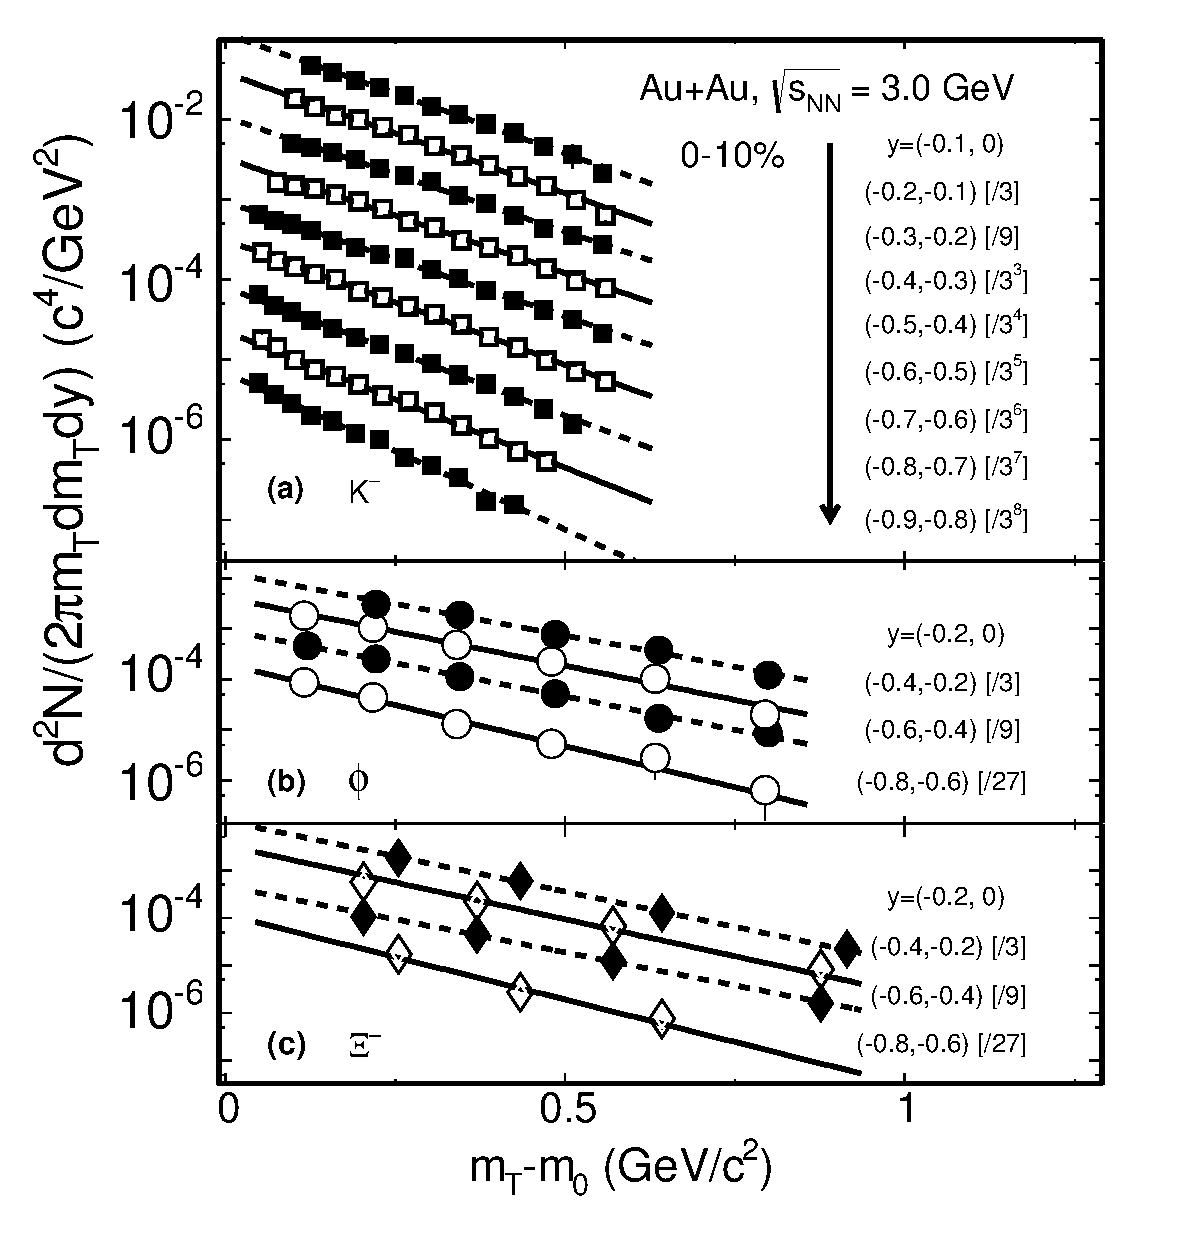
\includegraphics[width=0.43\textwidth]{fig21-eps-converted-to.pdf}
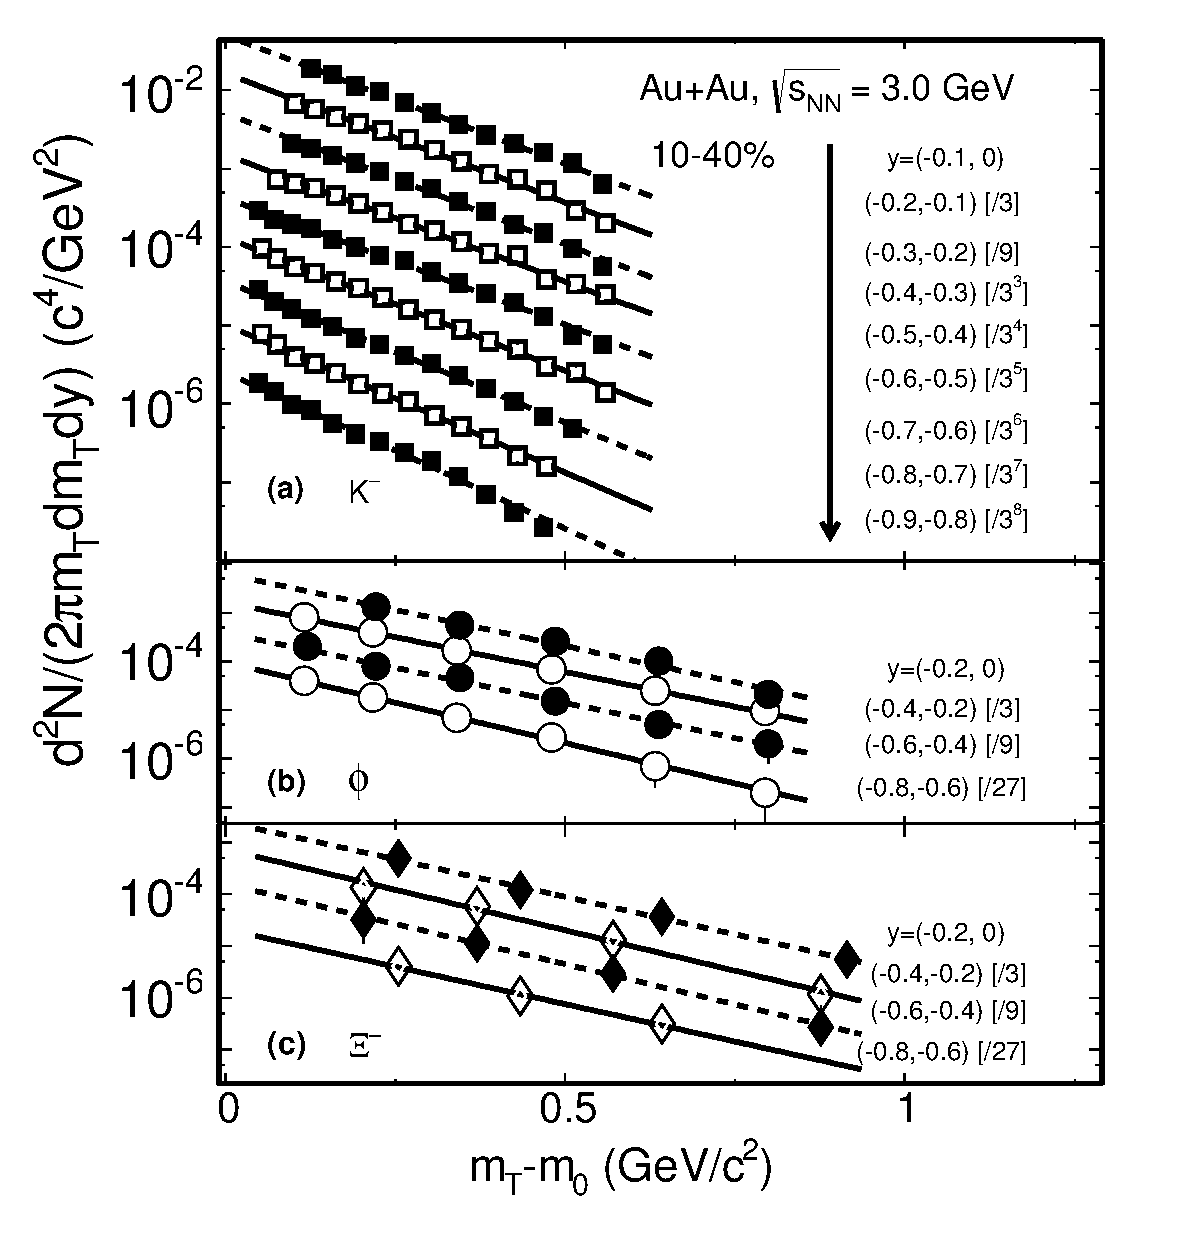
\includegraphics[width=0.43\textwidth]{fig22-eps-converted-to.pdf}
\caption{$K^-$ (a), $\phi$ meson (b) and $\Xi^-$ (c) invariant yields as a function of $m_T-m_0$ for various rapidity regions in 0--10\% (left) and  10--40\% (right) centrality Au+Au collisions at ${\sqrt{s_{\rm NN}} = \rm{3\,GeV}}$. Statistical and systematic uncertainties are added quadratically here for plotting. Solid and dashed black lines depict $m_T$ exponential function fits to the measured data points with scaling factors in each rapidity windows.}
\label{fig:phimTSpectra21}
\end{figure*}

\begin{figure}
\centering
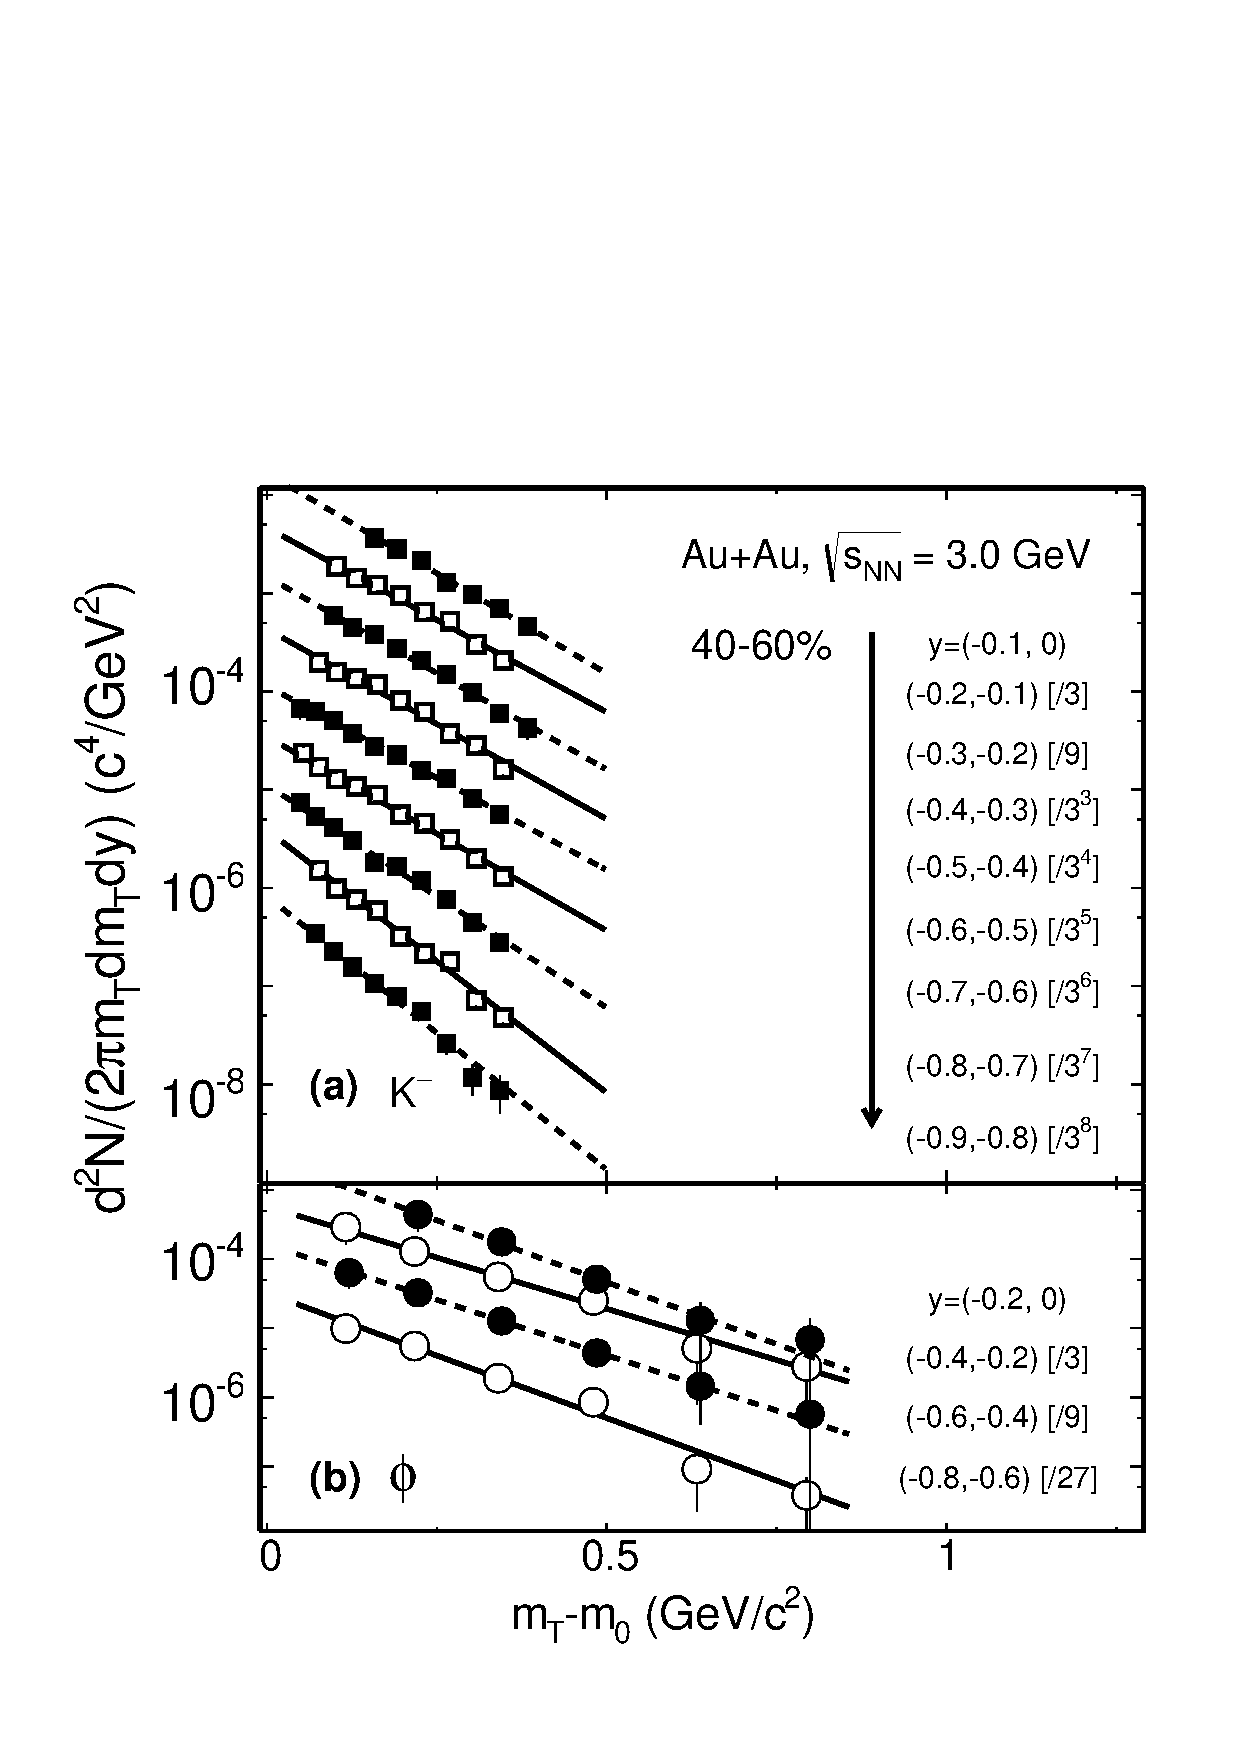
\includegraphics[width=0.43\textwidth]{fig23-eps-converted-to.pdf}
\caption{$K^-$ (a) and $\phi$ meson (b) invariant yields as a function of $m_T-m_0$ for various rapidity regions in 40--60\% centrality Au+Au collisions at ${\sqrt{s_{\rm NN}} = \rm{3\,GeV}}$.}
\label{fig:phimTSpectra23}
\end{figure}


\end{document}
